%import template
\documentclass[a4paper, landscape , 8pt]{scrartcl}

% use language german
\usepackage[T1]{fontenc}
\usepackage[utf8]{inputenc}
\usepackage[english, ngerman]{babel} % \selectlanguage{english} if  needed
\usepackage{lmodern} % use modern latin fonts

% format
\usepackage{geometry}
\geometry{top=1.2cm,left=0.4cm,right=0.4cm}
\textheight = 558pt

%autor
\usepackage{authblk}

%tabular
\usepackage{tabularx}

% math
\usepackage{amsmath}
\usepackage{amssymb}
\usepackage{amsfonts}
\usepackage{enumitem}

% graphic
\usepackage{graphicx}
\graphicspath{{graphic/}} 

%colors
% \usepackage{xcolor}

% Multi Columns
\usepackage{multicol}

% more compact items. explicit parameters as I want some separation between items
% see https://tex.stackexchange.com/questions/10684/vertical-space-in-lists
\setlist{topsep=0pt, leftmargin=4mm,itemsep=1.5pt,partopsep=0pt, parsep=0pt}
\setlength{\parindent}{0cm}

%define header and footer
\usepackage{fancyhdr}
\pagestyle{fancy}

\fancyhead[RO]{\AUTHOR| \INSTITUTE}
\fancyhead[LO]{\TITLE}
\fancyfoot[RO]{09.01.2022}
\renewcommand\headrulewidth{0pt}
\renewcommand\footrulewidth{0pt}
\headsep = -2pt
\footskip = 0pt


% Define Section Format
\usepackage{sectsty}
\usepackage{titlesec}
\usepackage[dvipsnames]{xcolor}

\titleformat{name=\section}[block]{\sffamily\normalsize}{}{0pt}{\colorsection}
\titlespacing*{\section}{0pt}{0pt}{0pt}
\newcommand{\colorsection}[1]{%
	\colorbox{sectioncolor!80}{\parbox{0.98\linewidth}{\vspace{-1pt}\color{white}\ #1 \vspace{-2pt}}}}

% Define Subsection Format
\titleformat{name=\subsection}[block]{\sffamily\small}{}{0pt}{\colorsubsection}
\titlespacing*{\subsection}{0pt}{0pt}{0pt}
\newcommand{\colorsubsection}[1]{%
	\colorbox{subsectioncolor!80}{\parbox{0.98\linewidth}{\vspace{-1pt}\color{black}\ #1 \vspace{-2pt}}}}

% Define SubSubsection Format
\titleformat{name=\subsubsection}[block]{\sffamily\small}{}{0pt}{\colorsubsubsection}
\titlespacing*{\subsubsection}{0pt}{0pt}{0pt}
\newcommand{\colorsubsubsection}[1]{%
	\colorbox{subsubsectioncolor!60}{\parbox{0.98\linewidth}{\vspace{-1pt}\color{black}\ #1 \vspace{-2pt}}}}


%define color
\definecolor{sectioncolor}{HTML}{052639}
\definecolor{subsectioncolor}{HTML}{468189}
\definecolor{subsubsectioncolor}{HTML}{8DB9B1}
\definecolor{b}{RGB}{0, 115, 192 } %Default highlight color
\definecolor{p}{RGB}{0, 43, 54} %Dark page color
\definecolor{t}{RGB}{131, 148, 150} %Dark text color
\definecolor{darkgreen}{RGB}{0,150,0}
\definecolor{dkgreen}{rgb}{0,0.6,0}
\definecolor{gray}{rgb}{0.5,0.5,0.5}
\definecolor{mauve}{rgb}{0.58,0,0.82}
\definecolor{DarkPurple}{rgb}{0.4, 0.1, 0.4}
\definecolor{DarkCyan}{rgb}{0.0, 0.5, 0.4}
\definecolor{LightLime}{rgb}{0.3, 0.5, 0.4}
\definecolor{Blue}{rgb}{0.0, 0.0, 1.0}
\definecolor{h}{RGB}{1, 101, 163}

% Code Listings
\usepackage{listings}
\usepackage{color}
\usepackage{beramono}
\usepackage{hyperref}
\hypersetup{
    colorlinks,
    linkcolor={black},
    citecolor={blue!50!black},
    urlcolor={blue!80!black}
}

\definecolor{bluekeywords}{rgb}{0,0,1}
\definecolor{greencomments}{rgb}{0,0.5,0}
\definecolor{redstrings}{rgb}{0.64,0.08,0.08}
\definecolor{xmlcomments}{rgb}{0.5,0.5,0.5}
\definecolor{types}{rgb}{0.17,0.57,0.68}

\lstdefinestyle{eclipse-style}{
	language=Java,
	showstringspaces=false,     
	basicstyle=\ttfamily\scriptsize,
	keywordstyle=\color{RoyalBlue}\ttfamily,
    stringstyle=\color{darkgreen}\ttfamily,
	commentstyle=\color{DarkPurple!60}\ttfamily,
	escapeinside={£}{£}, % latex scope within code      
	breaklines=true,
	breakatwhitespace=true,
	showspaces=false,
	showtabs=false,
	tabsize=2,
	morekeywords={length},
	numbers=none,
	numberstyle=\tiny\color{black},
	frame=none,
	aboveskip = 0em,
	belowskip = 0em
}
\lstset{
	style=eclipse-style
	% literate=  % Allow for German characters in lstlistings.
	% {Ö}{{\"O}}1
	% {Ä}{{\"A}}1
	% {Ü}{{\"U}}1
	% {ü}{{\"u}}1
	% {ä}{{\"a}}1
	% {ö}{{\"o}}1}
}

% Theorems \begin{mytheo}{title}{label}
\usepackage{tcolorbox}
\tcbuselibrary{theorems}
\newtcbtheorem[number within=section]{definiton}{Definition}%
{fonttitle=\bfseries}{def}
\newtcbtheorem[number within=section]{remember}{Merke}%
{fonttitle=\bfseries}{rem}
\newtcbtheorem[number within=section]{hint}{Hinweis}%
{fonttitle=\bfseries}{hnt}

% new section -> new page
% \let\stdsection\section
% \renewcommand\section{\clearpage\stdsection}

% Front page
\newcommand{\AUTHOR}{M. Panchaud}
\newcommand{\INSTITUTE}{Ostschweizer Fachhochschule}

%dotted rule
\usepackage{dashrule}
\usepackage{tikz}
\usetikzlibrary{decorations.markings}
\newcommand{\drule}[3][0]{
	\tikz[baseline]{\path[decoration={markings,
	mark=between positions 0 and 1 step 2*#3
	with {\node[fill, circle, minimum width=#3, inner sep=0pt, anchor=south west] {};}},postaction={decorate}]  (0,#1) -- ++(#2,0);}}


%no indentation
\setlength{\parindent}{0cm}

% DocInfo
\newcommand{\SUBJECT}{}
\newcommand{\TITLE}{Cheat Sheet Objektorientierte Programmierung 2}

\begin{document}

%do multicols
\begin{multicols*}{4}
    \setlength{\columnseprule}{0.2pt}
		\footnotesize

% TODO improve places where columnbreaks are done as soon as content is pretty much final
\section{Big O}

    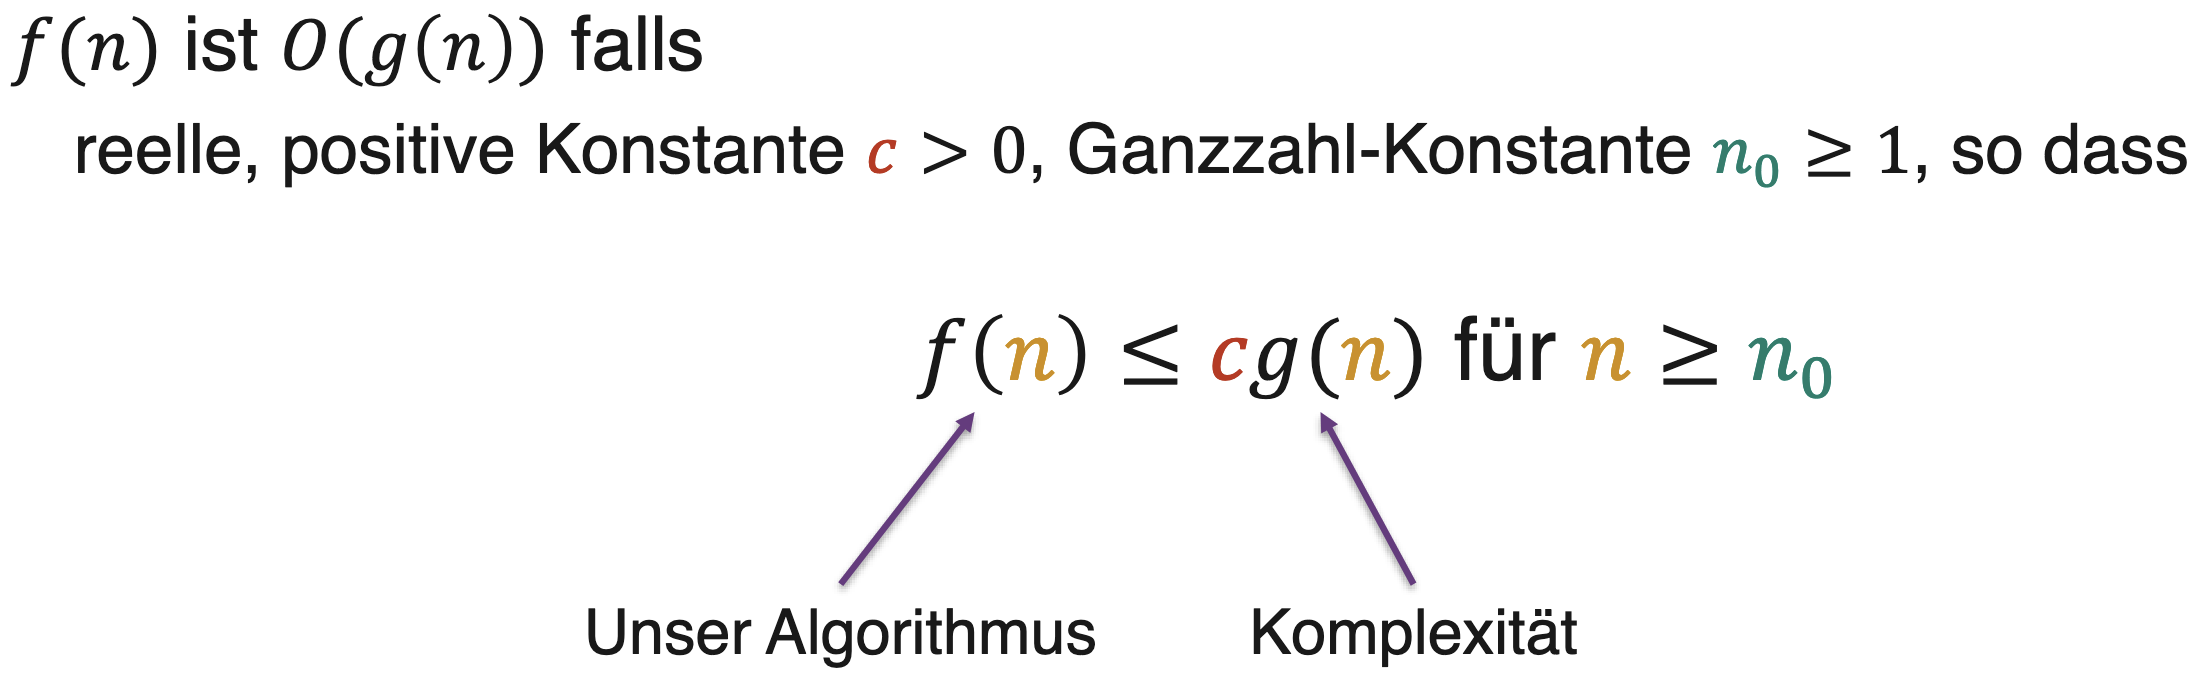
\includegraphics[scale=0.15]{graphic/14_big_o_notation_herleitung}
	\newline
	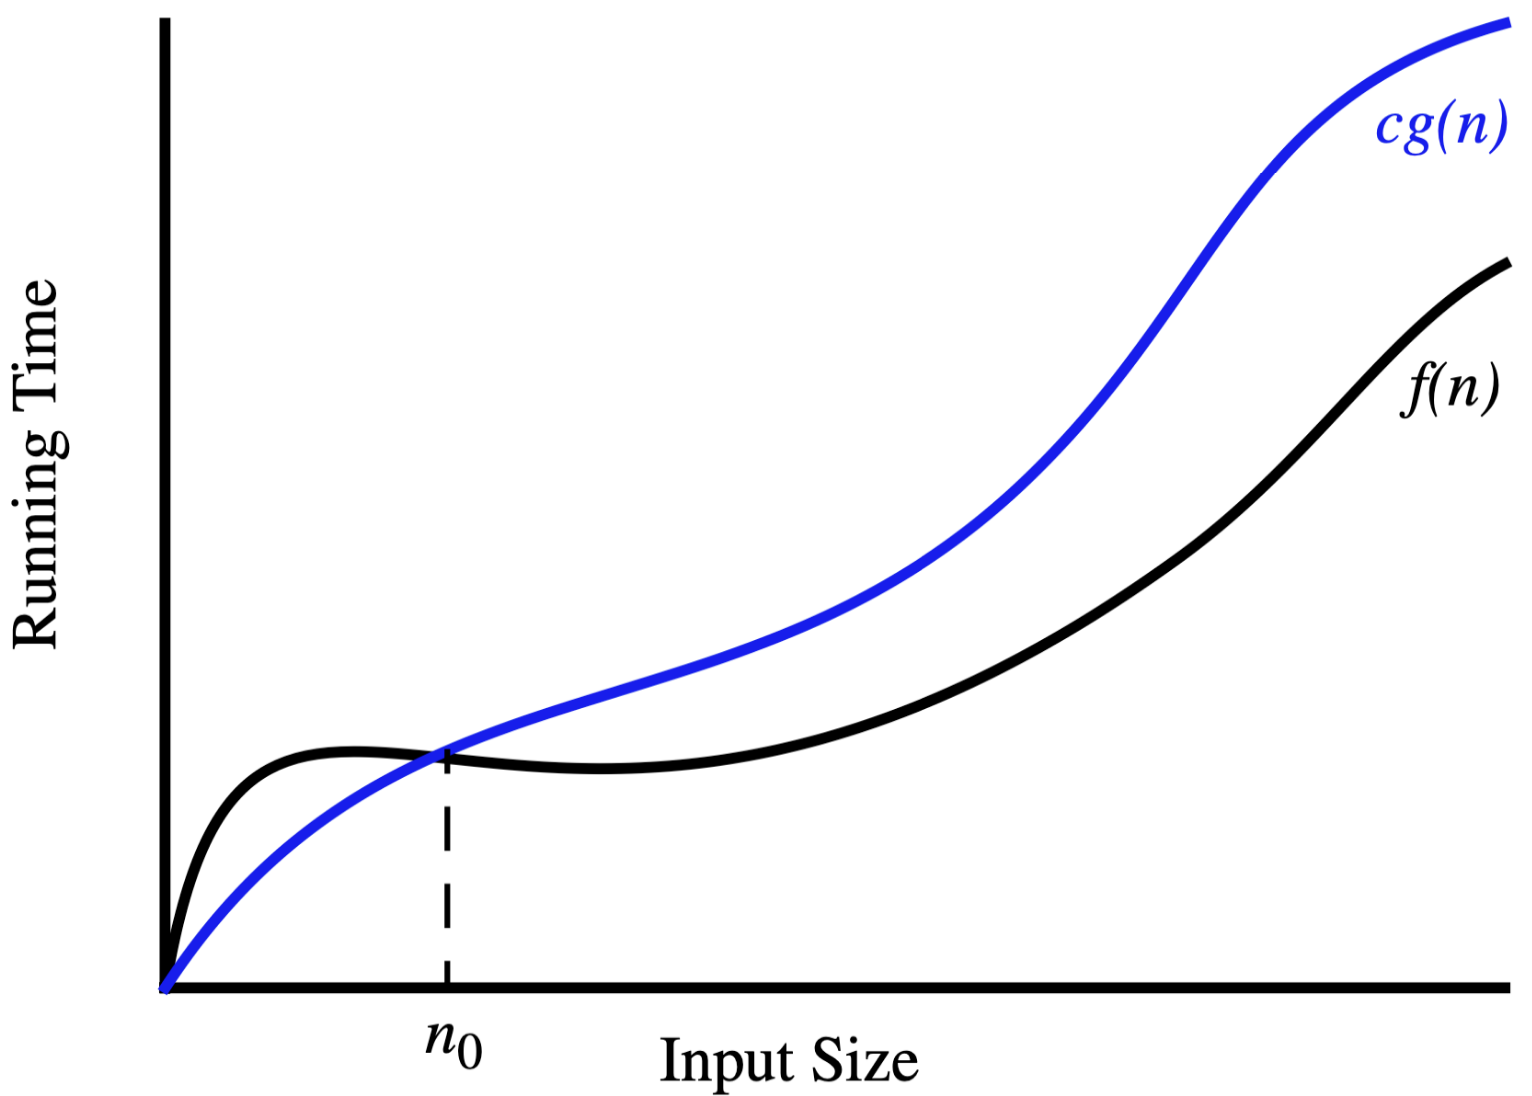
\includegraphics[scale=0.15]{graphic/03_big_o_notation}
	\newline
	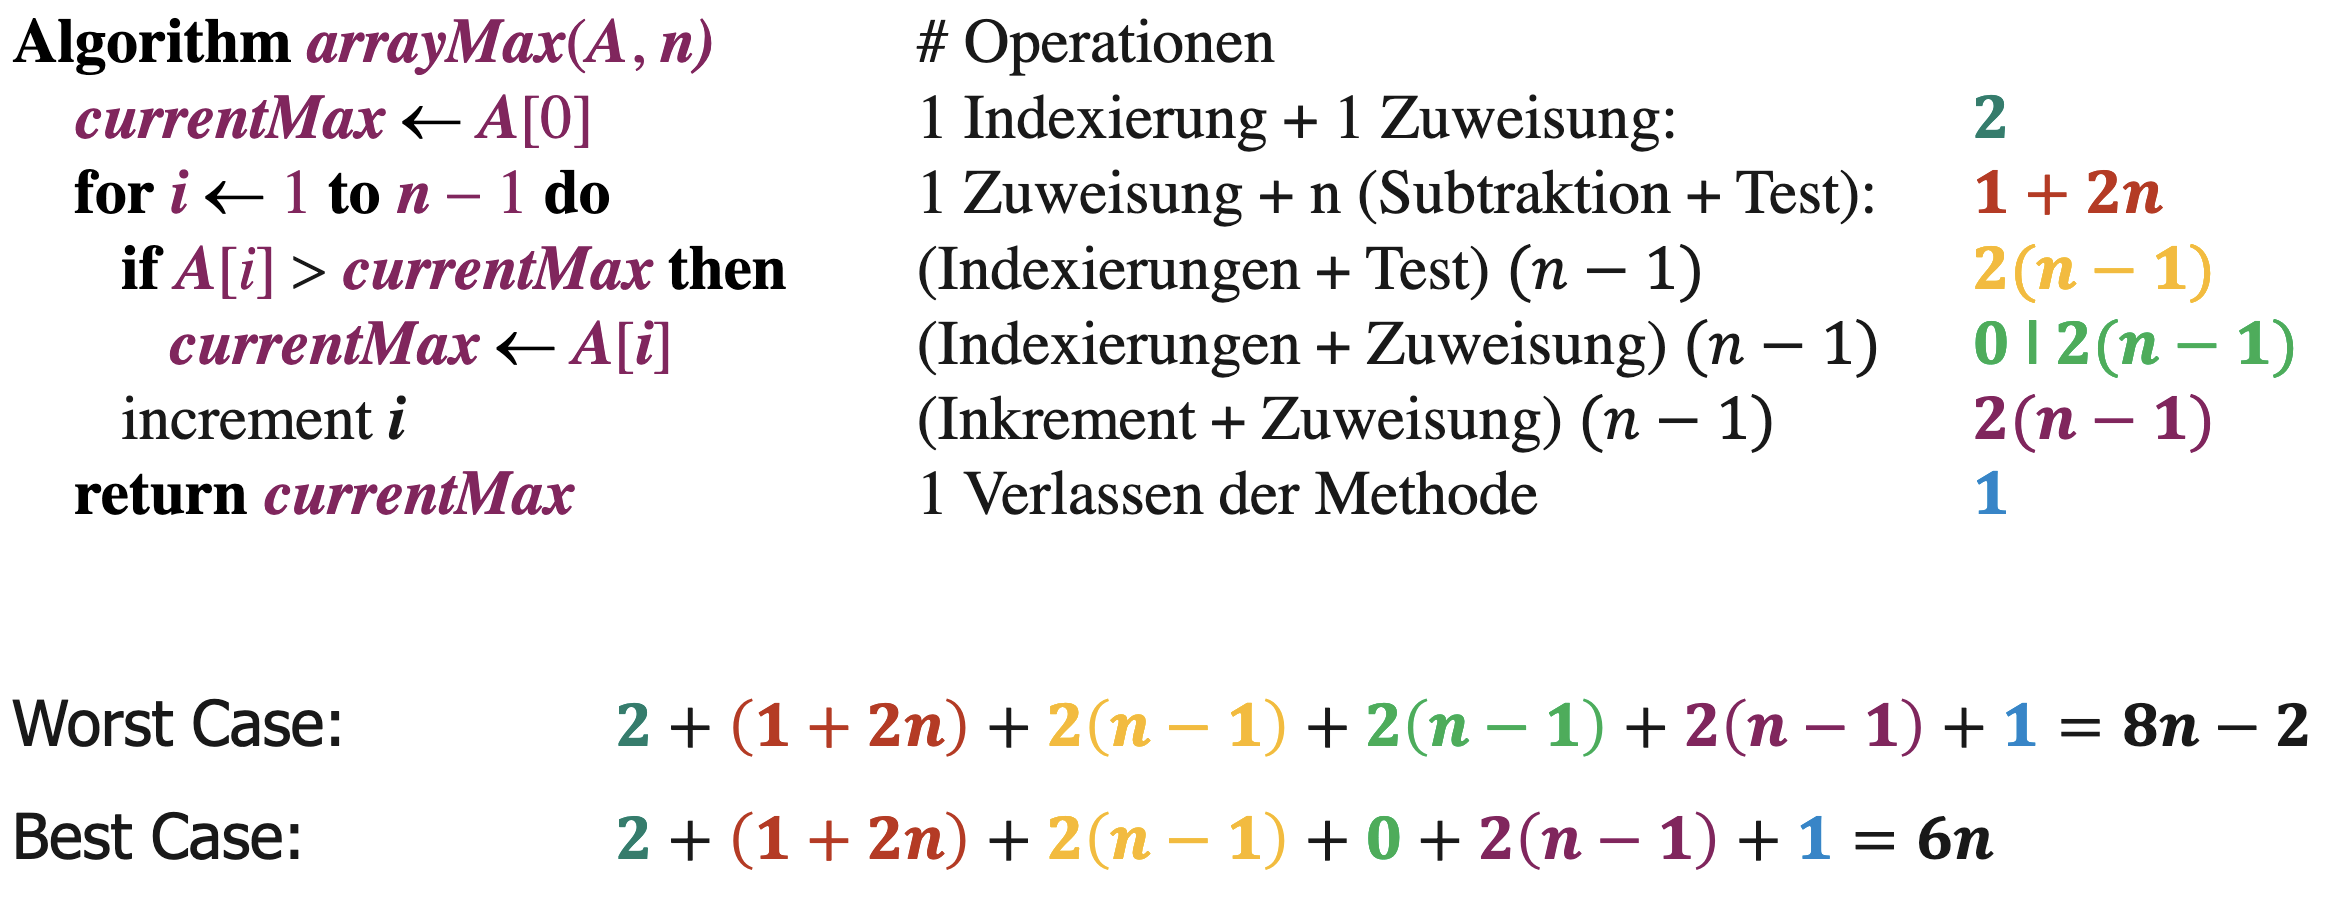
\includegraphics[scale=0.17]{graphic/04_primitive_operationen_zaehlen}

	\subsection{Beweis}
	\begin{itemize}
		\item Annahme: 2n + 10 ist O(n)
		\item $2n + 10 \leq cn$
		\item $10 \leq cn - 2n$
		\item $10 \leq (c - 2)n$
		\item $\frac{10}{c-2} \leq n$
		\item $=> c=3$ und $n0=10$
		\item Es gibt viele Belegungen für $c$ und $n0$
	\end{itemize}

	\subsection{Beispiel}
	\begin{lstlisting}
public static void function(int[] array) {
	// O(n)
	for (int i = 1; i < array.length + 1; i++) {
		// O(log n)
		for (int i1 = 1; i1 < array.length; i1*=2) {
			System.out.println(array[i - 1]);
		}
	}
}
// -> O(n * log n)
	\end{lstlisting}

\section{Verschiedene Algorithmen}
	\subsection{Eigenschaften}

	\renewcommand{\arraystretch}{1.1}
	\begin{tabular}{c | c | c | c}
		Algo & Worst & Avg & Best \\
		\hline
		Binary Search & O(log n) & O(log n) & O(1) \\
		Insertion & O($n^2$) & O($n^2$) & O(n) \\
		Selection & O($n^2$) & O($n^2$) & O($n^2$) \\
		Bubble & O($n^2$) & O($n^2$) & O(n) \\
		Merge & O(n log n) & O(n log n) & O(n log n) \\
		Quick & O($n^2$) & O(n log n) & O(n log n) \\
		Heap & O(n log n) & O(n log n) & O(n log n) \\
	\end{tabular}
	
	\subsection{Implementationen}
		\subsubsection{Binary Search}
		Nur wenn Array bereits sortiert ist. 
		
		Wiederholtes "halbieren" der möglichen Kandidaten.
		
		$ Pivot = \dfrac{low + high}{2}  $
		
		Wenn gesuchter Wert grösser als Pivot: Suche im rechten Teilbereich
		
		Wenn gesuchter Wert kleiner als Pivot: Suche im linken Teilbereich
		
		Wert gefunden: Abbruch und Rückgabe des Wertes
		
		\textbf{Rekursiv}
			\begin{lstlisting}
public int searchBinary(int[] intArr, int start, int end, int searchElement) {
	if (start > end || intArr.length == 0) {
		return null;
	}

	int pivot = (start + end) / 2);
	if (pivot >= intArr.length){
		return null;
	}
	if (searchElement > intArr[pivot]) {
		searchBinary(intArr, pivot + 1, end, searchElement);
	} else if (searchElement < intArr[pivot] && start != pivot) {
		searchBinary(intArr, start, pivot - 1, searchElement);
	} else if(searchElement == intArr[pivot]) {
		return intArr[pivot]
	} else{
		return null;
	} }
			\end{lstlisting}
		
		\textbf{Iterativ}
			\begin{lstlisting}
<T extends Comparable<T>> int searchBinaryIterative(List<? extends T> list, T searchElement) { 
	int start = 0; 
	int end = list.size() - 1; 
	while (start <= end) { 
		int pivot = start + ((end - start) / 2); 
		int compareResult = searchElement.compareTo(list.get(pivot)); 
		if (compareResult > 0) { 
			start = pivot + 1; 
		} else if (compareResult < 0) { 
			end = pivot - 1; 
		} else { 
			// index found 
			return pivot; 
		} 
	} 
	return -1; 
} 
			\end{lstlisting}
		
		\subsubsection{Insertion Sort}
		Für jedes neue Element wird geprüft, wo in der sortierten Liste es hingehört
			\begin{lstlisting}
void insertionSort(char[] data) {
	for (int k = 1; k < data.length; k++) {
		char cur = data[k];
		int j = k;
		while (j > 0 && data[j - 1] > cur) {
			data[j] = data[j - 1];
			j--;
		}
		data[j] = cur;
	} }
			\end{lstlisting}
		
		\subsubsection{Selection Sort}
		Kleinstes/grösstes Element suchen und an richtige Stelle verschieben
		
			\begin{lstlisting}
void selectionSort(int[] array) {
	int marker = array.length - 1;
	while (marker >= 0) {
		int max = 0;
		for (int i = 1; i <= marker; i++) {
			if (array[i] > array[max]) {
				max = i;
			}
		}
		swap(array, marker, max);
		marker--;
	} }
			\end{lstlisting}
		
		\subsubsection{Bubble Sort}
		Array von links nach rechts durchgehen, wenn Element grösser als rechter Nachbar, austausczhen
			\begin{lstlisting}
void bubbleSort(int[] array) {
	for (var n = array.length; n > 1; n--) {
		for (var i = 0; i < n - 1; i++) {
			if (array[i] > array[i + 1]) {
				swap(array, i, i + 1);
			}
		}
	} }
			\end{lstlisting}
		
		\subsubsection{Merge Sort}
		S auf Folgen S1 und S2 verteilen, rekursiv sortieren, S1 und S2 in sortierter Folge zusammenfassen
			\begin{lstlisting}
int[] mergeSort(int[] elem, int left, int right) {
	if (left == right)
	  	return new int[]{elem[left]};
	int middle = left + (right - left) / 2;
	int[] leftArray = mergeSort(elem, left, middle);
	int[] rightArray = mergeSort(elem, middle + 1, right);
	return merge(leftArray, rightArray);
}

int[] merge(int[] leftArray, int[] rightArray) {
	int leftLen = leftArray.length;
	int rightLen = rightArray.length;
	int[] target = new int[leftLen + rightLen];
	int targetPos = 0;
	int leftPos = 0;
	int rightPos = 0;// As long as both arrays contain elements...
	while (leftPos < leftLen && rightPos < rightLen) {
		// Which one is smaller?
		int leftValue = leftArray[leftPos];
		int rightValue = rightArray[rightPos];
		if (leftValue <= rightValue) {
			target[targetPos++] = leftValue;
			leftPos++;
		} else {
			target[targetPos++] = rightValue;
			rightPos++;
		}
	}
    // Copy the rest
	while (leftPos < leftLen) {
		target[targetPos++] = leftArray[leftPos++];
	}
	while (rightPos < rightLen) {
		target[targetPos++] = rightArray[rightPos++];
	}
	return target;
}
			\end{lstlisting}
		
		\subsubsection{Quick Sort}
		Pivot wählen, in zwei Arrays teilen, eines mit x < Pivot, eines mit x > Pivot, rekursiv auf Unterarrays Quicksort aufrufen
			\begin{lstlisting}
void quickSort(int[] arr, int low, int high) {
	if (low < high) {
		int pi = partition(arr, low, high);
		quickSort(arr, low, pi - 1);
		quickSort(arr, pi + 1, high);
	}
}
	
int partition(int[] arr, int low, int high) {
	int pivot = arr[high];
	int i = low - 1;
	for (int j = low; j <= high - 1; j++) {
		if (arr[j] < pivot) {
			i++;
			swap(arr, i, j);
		}
	}
	swap(arr, i + 1, high);
	return i + 1;
}
			\end{lstlisting}

		\subsubsection{Heap Sort}
			\begin{itemize}
				\item \textbf{max heap}: tree where parents are always > childs.
				\item \textbf{heapify}: creates max heap but assumes part of array is already sorted
				\item Build a max heap from the input data
				\item At this point, the largest item is stored at the root of the heap. Replace it with the last item of the heap followed by reducing the size of heap by 1, as this item is now sorted.
				\item Finally, heapify the root of tree.
				\item Repeat above steps while size of heap is greater than 1.			
			\end{itemize}
		
			\vspace{2pt}
			\begin{lstlisting}
public void sort(int arr[]) { 
	int n = arr.length; 
	// Build heap (rearrange array) 
	for (int i = n / 2 - 1; i >= 0; i--) {
		heapify(arr, n, i); 
	}
	// One by one extract an element from heap 
	for (int i = n - 1; i >= 0; i--) { 
		// Move current root to end 
		int temp = arr[0]; 
		arr[0] = arr[i]; 
		arr[i] = temp; 
		
		// call max heapify on the reduced heap 
		heapify(arr, i, 0); 
	} 
} 

// To heapify a subtree rooted with node i which is 
// an index in arr[]. n is size of heap 
void heapify(int arr[], int n, int i) { 
	int largest = i;  // Initialize largest as root 
	int l = 2 * i + 1;  // left = 2*i + 1 
	int r = 2 * i + 2;  // right = 2*i + 2 
	
	// If left child is larger than root 
	if (l < n && arr[l] > arr[largest]) {
		largest = l; 
	}
	
	// If right child is larger than largest so far 
	if (r < n && arr[r] > arr[largest]) {
		largest = r; 
	}
	
	// If largest is not root 
	if (largest != i) { 
		int swap = arr[i]; 
		arr[i] = arr[largest]; 
		arr[largest] = swap; 
		
		// Recursively heapify the affected sub-tree 
		heapify(arr, n, largest); 
	} 
} 
			\end{lstlisting}

		
		
\section{Bäume}
	\begin{itemize}
		\item \textbf{innerer Knoten}: Knoten mit min. einem Kind
		\item \textbf{Blatt}: Knoten ohne Kinder
		\item \textbf{Wurzel}: Knoten ohne Elternknoten
		\item \textbf{Geschwister}: Knoten mit selben Eltern
		\item \textbf{Vorgängerknoten}: Eltern, Grosseltern, ...
	\end{itemize}

	Binary Tree: Jeder Knoten höchstens zwei Kinder \& Kinder sind geordnetes Paar

	\subsection{Höhe}
	Maximale Tiefe der Knoten im Baum
		\begin{lstlisting}
public int height(Position<E> p) {
	int h = 0;
	for (Position<E> c : children(p)) {
		h = Math.max(h, 1 + height(c));
	}
	return h; }
		\end{lstlisting}
	
	\subsection{Tiefe}
	Anzahl Vorgänger
		\begin{lstlisting}
public int depth(Position<E> p) {
	if (isRoot(p)) {
		return 0;
	} else {
		return 1 + depth(parent(p));
	} }
		\end{lstlisting}
	\subsection{Traversierung}
		\subsubsection{Preorder W-L-R}
			\begin{lstlisting}
visit(v)
for each child w of v
  preOrder(w)
			\end{lstlisting}
		
		\subsubsection{Postorder L-R-W}
			\begin{lstlisting}
for each child w of v
  postOrder(w)
visit(v)
			\end{lstlisting}
		
		\subsubsection{Breadth-First}
		Alle Knoten der Tiefe t besuchen, bevor Knoten der Tiefe t+1 besucht werden
			\begin{lstlisting}
// Initialize queue Q containing root
while Q not empty
  v = Q.dequeue()
  visit(v)
  for each child w in children(v)
    Q.enqueue(w)
			\end{lstlisting}
		
		\subsubsection{Inorder L-W-R}
			\begin{lstlisting}
if hasLeft(v)
  inOrder(left(v))
visit(v)
if hasRight(v)
  inOrder(right(v))
			\end{lstlisting}

	\subsection{Preorder Iterator}
		\begin{lstlisting}
public T next() {
	if (stack.empty()) {
		stack.push(root);
	}
	Node<T> node = stack.pop();
	if (node.getRight() != null) {
		stack.push(node.getRight());
	}
	if (node.getLeft() != null) {
		stack.push(node.getLeft());
	}
	if (stack.empty()) {
		root = null;
	}
	return node.getValue(); 
}
		\end{lstlisting}

\section{Algorithmenparadigmen}
 \textbf{Algorithmus: Präzise endliche Beschreibung eines allgemeinen Verfahrens unter Verwendung
	ausführbarer elementarer Schritte}

	\subsection{Backtracking}
		\subsubsection{Cookbook}
			\renewcommand{\outlineii}{enumerate}
			\renewcommand{\outlineiii}{enumerate}
			\begin{outline}
				\1 Position markieren
				\1 Rekursionsabbruch (zB alles besucht, Ausgang gefunden): return true 
				\1 Alle Optionen probieren
					\2 neues Feld festlegen
					\2 Überprüfen ob gültig \& nicht besucht
						\3 Wenn ja: prüfen ob rekursiver Aufruf true? 
							\4 Wenn ja: return true
				\1 Backtracking: Markierung vom Feld entfernen und return false
			\end{outline}
			\renewcommand{\outlineii}{itemize}
			\renewcommand{\outlineiii}{itemize}
		
		\subsubsection{Beispiel Knights Tour}
			\begin{lstlisting}
boolean isValid(int x, int y) {
	return x >= 0 && y >= 0 && x < N && y < N;
}

boolean knightTour(int[][] visited, int x, int y, int pos) {
	// jetzige Position markieren
	visited[x][y] = pos;
	// alle Felder besucht => abbrechen (return true)
	if (pos >= N * N) {
		print(visited);
		return true;
	}
	// Alle erlaubten Bewegungen überprüfen
	for (int k = 0; k < 8; k++) {
		int newX = x + row[k];
		int newY = y + col[k];
		// neue Position auf Feld und noch nicht besucht
		if (isValid(newX, newY) && visited[newX][newY] == 0) {
			// Wenn die Rekursion ein Weg gefunden hat
			if (knightTour(visited, newX, newY, pos + 1)){
				return true;
			}
		}
	}
	
	// Markierung entfernen und backtracken
	visited[x][y] = 0;
	return false;
}
			\end{lstlisting}
		
		\subsubsection{Beispiel Sudoku Solver}
			\begin{lstlisting}
public class SudokuSolver { 
	public static final int size = 9; 
	
	boolean isNumberUsedInRow(int[][] fields, int row, int number) { 
		for(int i = 0; i < size; i++) { 
			if(fields[row][i] == number) { 
				return true; 
			} 
		} 
		return false; 
	} 
	
	boolean isNumberUsedInCol(int[][] fields, int col, int number) { 
		for(int i = 0; i < size; i++) { 
			if(fields[i][col] == number) { 
				return true; 
			} 
		} 
		return false; 
	} 
	
	boolean isNumberUsedInSquare(int[][] fields, int row, int col, int number) { 
		// start at the top left value 
		col = col - (col % 3); 
		row = row - (row % 3); 
		for(int i = 0; i < 3; i++) { 
			for(int j = 0; j < 3; j++) { 
				if(fields[row + i][col + j] == number) { 
					return true; 
				} 
			} 
		} 
		return false; 
	} 
	
	boolean isNumberValid(int[][] fields, int row, int col, int number) { 
		return !isNumberUsedInRow(fields, row, number) && !isNumberUsedInCol(fields, col, number) && 
		!isNumberUsedInSquare(fields, row, col, number); 
	} 
	
	private int[] getNextFreeField(int[][] fields) { 
		for(int i = 0; i < size; i++) { 
			for(int j = 0; j < size; j++) { 
				if(fields[i][j] == 0) { 
					return new int[]{i,j}; 
				} 
			} 
		} 
		return new int[0]; 
	} 
	
	public boolean solveSudoku(int[][] fields) { 
		int[] freeField = getNextFreeField(fields); 
		if(freeField.length == 0) { 
			return true; 
		} 
		int x = freeField[0]; 
		int y = freeField[1]; 
		
		for(int i = 1; i < size+1; i++) { 
			if(isNumberValid(fields, x, y, i)) { 
				fields[x][y] = i; 
				if(solveSudoku(fields)) { 
					return true; 
				} 
			} 
			
		} 

		fields[x][y] = 0; 
		return false; 
	} 
} 
			\end{lstlisting}

	\subsection{Greedy}
	Lösung wählen, die im Teilschritt möglichst nahe ans Ziel kommen.
	Beispiel Rückgeld: Grösste Münze von Betrag abziehen

	\subsubsection{Set-Covering Problem}
	\textcolor{subsectioncolor}{Beispiel Abdeckung Radiostationen in den USA}
	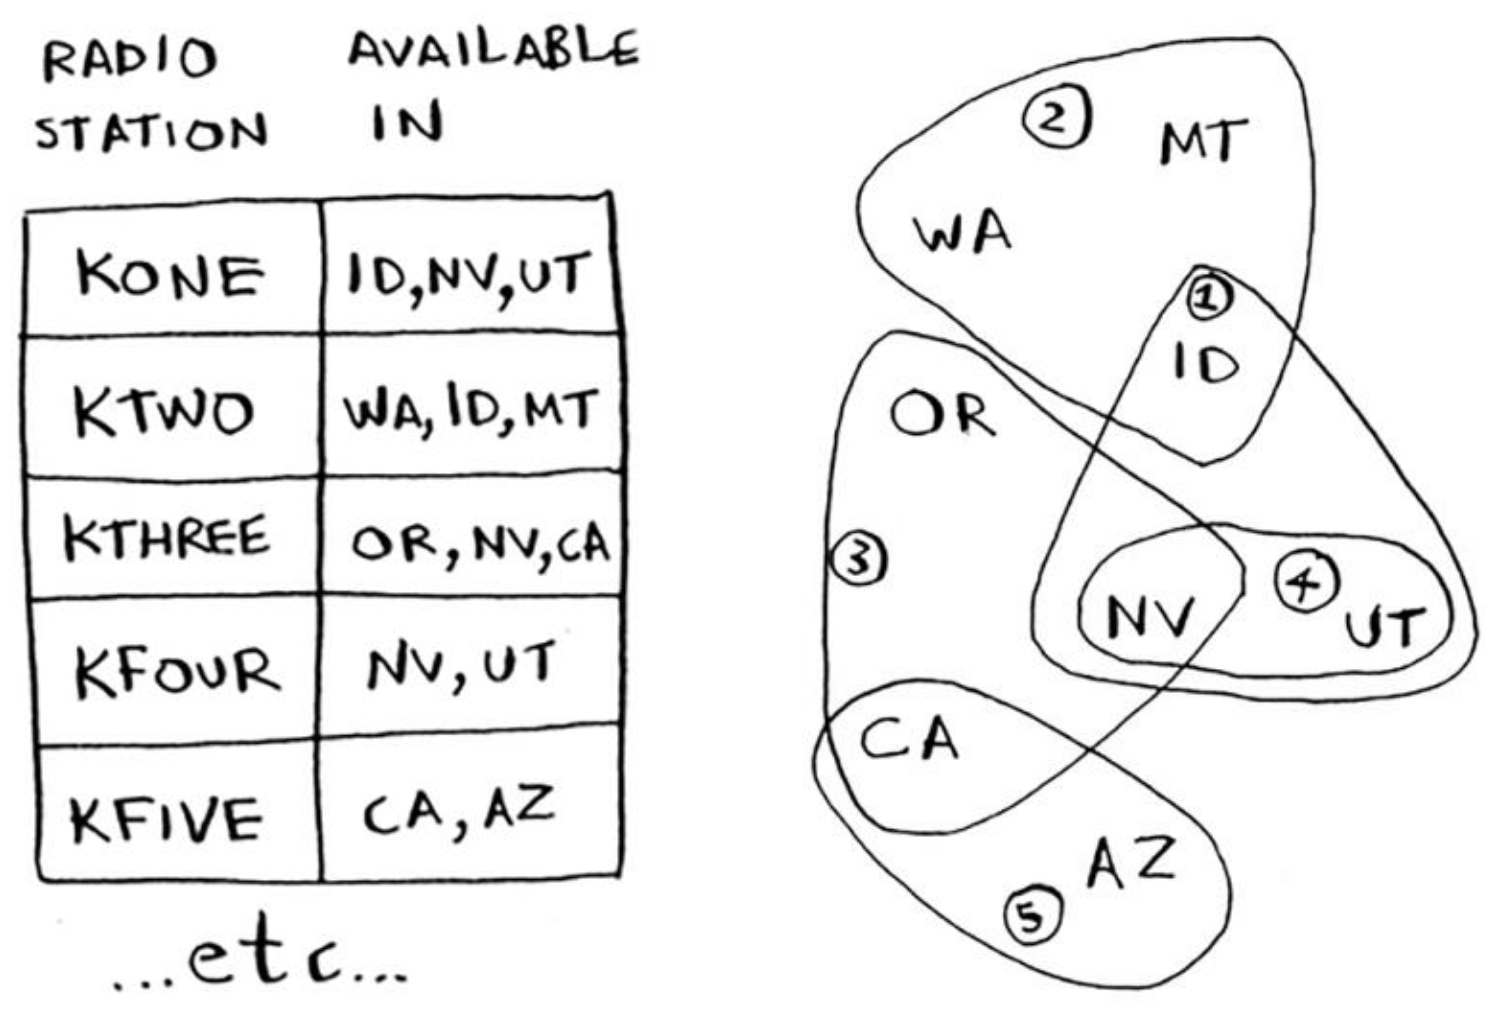
\includegraphics[scale=0.15]{graphic/08_set_covering_radio_stations}
		\begin{itemize}
			\item Optimaler Algorithmus
			\begin{itemize}
				\item Alle Teilmengen der Stationen aufzählen
				\item Minimale Anzahl Stationen wählen
				\item {\bfseries Problem:} $2^n$ mögliche Kombinationen (Potenzmenge)
			\end{itemize}
		\end{itemize}
		{\bfseries $\to$ Es gibt keinen Algorithmus, der Problem schnell genug löst}
		\newline
		\textcolor{subsectioncolor}{Alternative}
		\begin{itemize}
			\item Wähle Sender, der meisten Sender abdeckt, die noch nicht abgedeckt sind
			\item Widerholen, bis alle Sender abgedeckt sind
		\end{itemize}
		\begin{lstlisting}
public static void calculateSolution(HashSet<String> statesNeeded, HashMap<String, HashSet<String>> stations) {
	var finalStations = new HashSet<String>();
	while (!statesNeeded.isEmpty()) {
		String bestStation = "";
		var statesCovered = new HashSet<String>();
		for (String station : stations.keySet()) {
			var covered = new HashSet<String>(statesNeeded);
			covered.retainAll(stations.get(station));
			if (covered.size() > statesCovered.size()) {
				bestStation = station;
				statesCovered = covered;
			}
		}
		statesNeeded.removeAll(statesCovered);
		finalStations.add(bestStation);
	}
	System.out.println(finalStations);
}
		\end{lstlisting}

	\subsection{Teile \& Herrsche}
		\begin{itemize}
			\item Problem aufteilen
			\item Kleinere Probleme lösen
			\item Rekursive Rückführung des Problems auf identisches Problem mit kleinerer Eingabemenge
		\end{itemize}
	
	\subsection{Dynamische Programmierung}
		\begin{itemize}
			\item Greedy
			\item Mehrfach auftretende Probleme nur einmal berechnen
			\item Lösung auf Grundlage bereits berechneter Ergebnisse finden
		\end{itemize}

\section{Rekursion}
	\begin{outline}
		\1 Rekursive Aufrufe werden auf Call Stack gelegt, bis Base Case erreicht
		\2 Aufrufe führen Richtung Base Case
		\1 Base Case erreicht
		\2 Rekursion bricht ab
		\2 Wert wird zurückgegeben
		\2 Abarbeiten der Stack Frames
	\end{outline}

	\subsection{Cookbook}
		\begin{itemize}
			\item Was ist der Base Case?
			\item Wie kann das Problem verkleinert werden?
		\end{itemize}
	
	\subsection{Arten}
		\begin{itemize}
			\item Lineare Rekursion: Rekursion macht höchstens einen weiteren Aufruf
			\item Binäre Rekursion: Wenn zwei rekursive Aufrufe in allen nicht-terminalen Aufrufen ausgeführt werden
			\item Endrekursion: Rekursiver Aufruf ist \underline{letzte} Anweisung in der Funktion
		\end{itemize}

 	\subsubsection{NDigitNums}
		\begin{lstlisting}
public static void findNDigitNums(String currentNumber, int n, int target, List<Integer>
resultList) {
	if (n > 0 && target >= 0) {
		char digit = '0';
		if (currentNumber.equals("")) {
			digit = '1';
		}
		while (digit <= '9') {
			String num = currentNumber + digit;
			int newTarget = target - (digit - '0');
			findNdigitNums(num, n-1, newTarget, resultList);
			digit++;
		}
	} else if (n == 0 && target == 0) {
		resultList.add(Integer.valueOf(currentNumber));
	}
}
		\end{lstlisting}

	\subsection{Endrekursion}
	Weniger Speicher benötigt.
		\begin{lstlisting}
private static int tailrecsum(int x, int total) {
	if (x == 0) {
		return total;
	} else {
		// Rekursiver Aufruf ist letzte Anweisung!
		return tailrecsum(x - 1, total + x);
	}
}

// Ohne Endrekursion
private static int recsum(int x) {
	if (x == 0) {
		return 0;
	} else {
		// Addition ist letzte Anwesiung!
		return x + recsum(x - 1);
	}
}
		\end{lstlisting}

\section{Abstrakter Datentyp}
Beschreibt Datenstruktur unabhängig von konkreter Implementierung.
Beschreibt Attribute, Operationen auf den Attributen, Ausnahmen und Fehler
Beschreibt das Was aber nicht das Wie.

\subsection{Datenstrukturen}
	\begin{itemize}
		\item Speichern und organisieren Daten.
		\item Implementieren einen ADT (Schnittstelle)
	\end{itemize}

	\subsubsection{Laufzeiten}

		\begin{tabular}{c | c | c}
			& Array & Linked List \\
			\hline
			Lesen & O(1) & O(n) \\
			Einfügen & O(n) & O(1)  \\
			Suchen & O(n) & O(n) \\
		\end{tabular}
	
		\begin{tabular}{c | c | c}
			\textbf{HashMap} & Avg & Worst \\
			\hline
			Lesen & O(1) & O(n) \\
			Einfügen & O(1) & O(n)  \\
			Suchen & O(1) & O(n) \\
		\end{tabular}

\section{Queue}
	\begin{itemize}
		\item enqueue(E): Element am Ende einfügen
		\item Object dequeue(): Element vom Anfang entfernen und
		zurückgeben
		\item E first(): liefert erstes Element, ohne es zu entfernen
		\item integer size(): Gespeicherte Elemente
		\item boolean isEmpty(): ist Queue leer?
	\end{itemize}

	\subsection{Priority Queue}
		\begin{itemize}
			\item insert(k, v): Fügt Eintrag mit Schlüssel k und Wert v ein
			\item removeMin(): Entfernt Eintrag mit kleinstem Schlüssel und gibt ihn zurück
			\item min(): Liefert Eintrag mit kleinstem Schlüssel, ohne diesen zu entfernen
			\item size(): Anzahl Elemente in Queue
			\item isEmpty(): Sind Elemente in der Queue?
		\end{itemize}
		
		\begin{tabular}{c | c | c}
			\textbf{Methode} & \textbf{Unsorted List} & \textbf{Sorted List} \\
			\hline
			\textbf{size} & O(1) & O(1) \\
			\textbf{isEmpty} & O(1) & O(1) \\
			\textbf{insert} & O(1) & O(n) \\
			\textbf{min} & O(n) & O(1) \\
			\textbf{removeMin} & O(n) & O(1) \\
		\end{tabular}
	
	Sorted
	\begin{lstlisting}
public class SortedPriorityQueue<K,V> extends AbstractPriorityQueue<K,V>  {
	// size left out as its just list.size()
	
	public Entry<K, V> insert(K key, V value) {		
		checkKey(key);
		var newest = new PriorityQueueEntry<>(key, value);
		
		if (list.size() == 0) {
			list.add(newest);
			return newest;
		}
		
		Entry<K,V> walk = list.get(list.size() - 1);
		int index = 0;
		
		for (index = list.size() - 1; index >= 0 && compare(newest, walk) > 0; index--) {
			walk = list.get(index);	
		}
		
		if (index == -1) {
			list.add(newest);
		} else {
			list.add(index, newest);
		}
		return newest;
	}
	
	public Entry<K, V> min() {
		return list.get(0);
	}
	
	public Entry<K, V> removeMin() {
		return list.remove(0);
	}
}
	\end{lstlisting}

	Unsorted
	\begin{lstlisting}
public class UnsortedPriorityQueue<K,V> extends AbstractPriorityQueue<K,V> {
	// size left out as its just return list.size()
	
	private Entry<K,V> findMin() {
		Entry<K,V> small = list.get(0);
		for (Entry<K,V> walk : list) {
			if (compare(walk, small) < 0) {
				small = walk;
			}
		}
		return small;
	}
	
	public Entry<K,V> insert(K key, V value) throws IllegalArgumentException {
		checkKey(key);
		Entry<K,V> newest = new PriorityQueueEntry<>(key, value);
		list.add(newest);
		return newest;
	}

	public Entry<K,V> min() {
		if (list.isEmpty()) {
			return null;
		}
		return findMin();
	}

	public Entry<K,V> removeMin() {
		if (list.isEmpty()) {
			return null;
		}
		var entry = findMin();
		list.remove(entry);
		return entry;
	}
}
	\end{lstlisting}

\section{Design Patterns}
	Arten von Design Patterns
	\begin{itemize}
		\item \textbf{Erzeugunsmuster}: Abstrahieren Instanziierung 
		\item => (Factory, Singleton, ...)
		\item \textbf{Strukturmuster}: Zusammensetzung von Klassen \& Objekten zu grösseren Strukturen
		\item => Adapter, Fassade, ...
		\item \textbf{Verhaltensmuster}: Algorithmen und Verteilung von Verantwortung zwischen Objekten
		\item => Iterator, Visitor, ...
	\end{itemize}
	\subsection{Iterator}
	Sequentiell auf Elemente in Aggregatobjekt zugreifen, ohne zugrundeliegende Struktur offen zu legen
	
	\subsection{Adapter}
	Klasse modifizieren, dass Schnittstelle zu Schnittstelle der anderen Klasse passt.
	
	Ermöglicht Code wieder zu verwenden ohne anzupassen.
	
	Objekt Adapter:
	\begin{lstlisting}
class Adapter extends ClassWeWantToMatch {
	private ExistingClass obj;
	public void method() {
		obj.otherMethod();
	}
}
	\end{lstlisting}

	\subsection{Template}
	\begin{itemize}
		\item Gemeinsame unveränderlichen Teile in abstrakter Klasse implementiert
		\item Variable Schritte werden in Methode ausgelagert
		\item Variable Schritte repräsentieren Hooks/Platzhalter, die in konkreten Subklassen implementiert werden.
	\end{itemize}

	\subsection{Visitor}
	Beschreibt Operationen auf Elementen einer anderen Datenstruktur.
	
	Trennung von Algorithmen und Datenstrukturen auf denen sie operieren. 
	
	Visitor enthält Algorithmen für unterschiedliche Datenstrukturen.
	\begin{itemize}
		\item \textbf{Einfache} Erweiterbarkeit, wenn neue Algorithmen hinzugefügt werden
		\item \textbf{Grösserer} Änderungsbedarf, wenn neue Klassen ergänzt werden
	\end{itemize}

\section{Hash}

	\subsection{Eigenschaften guter Hashfunktionen}
	\begin{itemize}
		\item konsistente Ergebnisse
		\item konstanter Zeitbedarf
		\item Gleichmässige Verteilung der Schlüssel
	\end{itemize}

	\subsection{Mögliche Hash Algorithmen}
		\subsubsection{Integer Cast}
		Schlüssel als Integer interpretieren
		
		• Gut, wenn Anzahl Bits Interpretation als Integer erlaubt
	
		\subsubsection{Komponentensumme}
		• Bits des Schlüssels in Komponenten fixer Länge (16/32 Bits) unterteilen
		
		• Komponenten summieren, Overflow ignorieren
		
		• Gut für Schlüssel fixer Länge, grösser/gleich Anzahl Bits von Integer
		
		\begin{lstlisting}
int hash = 0;
for (int i = 0; i < s.length(); i++) {
	hash = (R * hash + s.charAt(i)) % m;
	// R ist Konstante. Eine kleine Primzahl
}
		\end{lstlisting}	
	
	\subsection{Polynom-Akkumulation}
	• Hashing von Werten der Form ($x_0, x_1 , ..., x_n-1$) schwierig durch Addition
	
	Polynom:
	$p(z) = a_0 + a_1z + a_2z^2 + ... + a_{n-1}$
		
	Gut für Strings. Mit z=33 maximal 6 Kollisionen bei 50'000 englischen Wörtern.

	\subsection{Erweiterbares Hashing}
	Beim erweiterbaren Hashing wird binäres Ergebnis der Hashfunktion verwendet, die auf einen grösaseren Bereich abbildet.
	
	Beim Überlauf eines Behälters wird ein weiteres Bit des Hashwertes hinzugezogen.
	
	Somit ist keine Reorganisation der gesamten Tabelle notwendig.
		
	\subsection{Kollisionsbehandlung}
		\subsubsection{Geschlossene Adressierung}
		Behälter von Map sind (verkettete) Listen
		
		Platz nicht begrenzt, Prinzipiell keine Überläufer
		
		\subsubsection{Offene Adressierung}
		Für Überläufer in anderen Behältern Platz suchen
		
		Sondierungsfolge bestimmt Weg zum Speichern und Wiederauffinden der Überläufer
		
		Lineare Sondierung: Überläufer in nächste verfügbar Zelle einfügen
		
		\textbf{Löschen}: Erfordert besondere Behandlung.
		
		Wird Datensatz gelöscht, kann dies Sondierungsfolge für anderen Datensatz unterbrechen.
		
		Datensätze nicht physisch löschen, sondern nur als gelöscht markieren. (Behälter ist: frei, belegt oder gelöscht)

\section{Generics}
Type Erasure!

Statisches Attribut kann nicht generisch sein.

=> Es wäre unklar, welchen Typ das statische Attribut tatsächlich hat, da Attribut zwischen Instanzen geteilt wird.

	\begin{tabular}{c | c}
		\textbf{Conventions} &  \\
		\hline
		T & Type \\
		K & Key \\
		V & Value \\
		N & Number \\
		E & Element \\
		S, U, V, ... & 2nd, 3rd, 4th \\
	\end{tabular}

	\begin{lstlisting}
Stack<String> genericStack = new Stack<String>();
Stack rawStack = genericStack;
// This works but loses type info, gives a warning
// Type only gets checked at runtime
	\end{lstlisting}

\vspace{5pt}

	\begin{lstlisting}
public class Stack<T> { ... }
interface Iterator<E> { ... }

// Class doesn't necessarily need to be generic
public <E> Stack<E> push(E value) { ... }
	\end{lstlisting}

	\subsection{Constraints}
		\begin{lstlisting}
... <T extends Graphic>

// Java doesn't allow Diamond inheritance: only one can be a class
... <T extends Type1 & Type2 & ... >

... <T super Graphic>
		\end{lstlisting}
	
	\subsection{Generische Type Invariance}
		\begin{lstlisting}
// This doesn't work. 
// Types need to be exactly the same
List<Number> ns = new ArrayList<Integer>();

Collection<? extends T> x = ....
Collection<? super T> y = ...
		\end{lstlisting}

% + just print the old cheatsheet again.

\end{multicols*}

% \appendix

% List of figures
\listoffigures

% List of tables
\listoftables

\end{document}